\documentclass[9pt]{extarticle}
\usepackage[margin=0.7in]{geometry}
\usepackage{graphicx}
\usepackage{booktabs}
\usepackage{hyperref}
\usepackage{float}
\usepackage{titlesec}
\usepackage{enumitem}
\usepackage{caption}

\setlength{\parindent}{0pt}
\setlength{\parskip}{4pt}
\setlength{\textfloatsep}{8pt plus 2pt minus 2pt}
\setlength{\floatsep}{8pt plus 2pt minus 2pt}
\setlength{\intextsep}{8pt plus 2pt minus 2pt}
\titlespacing*{\section}{0pt}{0.8em}{0.3em}
\titlespacing*{\subsection}{0pt}{0.5em}{0.2em}
\captionsetup{font=small}

\title{ComicTrans: Local Manga (Japanese comic) Translation}
\author{Rok Mušič}
\date{May 2026}

\begin{document}
\small
\maketitle
\vspace{-2.0em}

\section{Introduction}
Automatic translation of mangas is a difficult vision task. A useful system must first find text in a cluttered black and white page, then read stylized Japanese writing, translate short context dependent dialogue, remove the original text, and finally redraw readable English without destroying the artwork. This is harder than ordinary OCR or ordinary machine translation because manga combines vertical text, sound effects, unusual fonts, dense panel layouts, very small speech bubbles, and text not appearing inside speech bubbles.

Historically, this problem has usually been approached as a pipeline: text detection, OCR, machine translation, then some form of inpainting and redrawing. Recent research has moved toward data driven approaches and more multimodal solutions that use full page context rather than isolated text strings. For this project, I chose a modular local pipeline because it is easier to debug, easier to benchmark stage by stage, and practical to run without cloud services (it is also free and accessible!).

For anyone who reads manga, the motivation is clear: there are many great series that are not officially licensed in English, and fan translations are often the only way to read them. A good automatic system could make these stories more accessible to a wider audience, especially in cases when not even fan translations exist. Another reason is language learning: a user can translate a manga into the language they are learning, or contrast the translation with the original if learning Japanese. For the research community, manga translation could be an interesting test case for multimodal use, OCR in the wild, and context aware machine translation.

\section{Pipeline overview}
The system has four stages: \textbf{(1)} detect and transcribe Japanese text regions with a multimodal (vision) OCR model PaddleOCR-VL, \textbf{(2)} translate the extracted text to English with a local LLM Gemma 4 served through \texttt{llama.cpp}, \textbf{(3)} remove the original text regions, and \textbf{(4)} redraw the English text inside those regions. Figure~\ref{fig:aotthreeway} compares three final translated versions of the same \emph{Attack on Titan} page, while Figure~\ref{fig:pipeline} shows the internal stages of my pipeline on that page.

\begin{figure}[H]
    \centering
    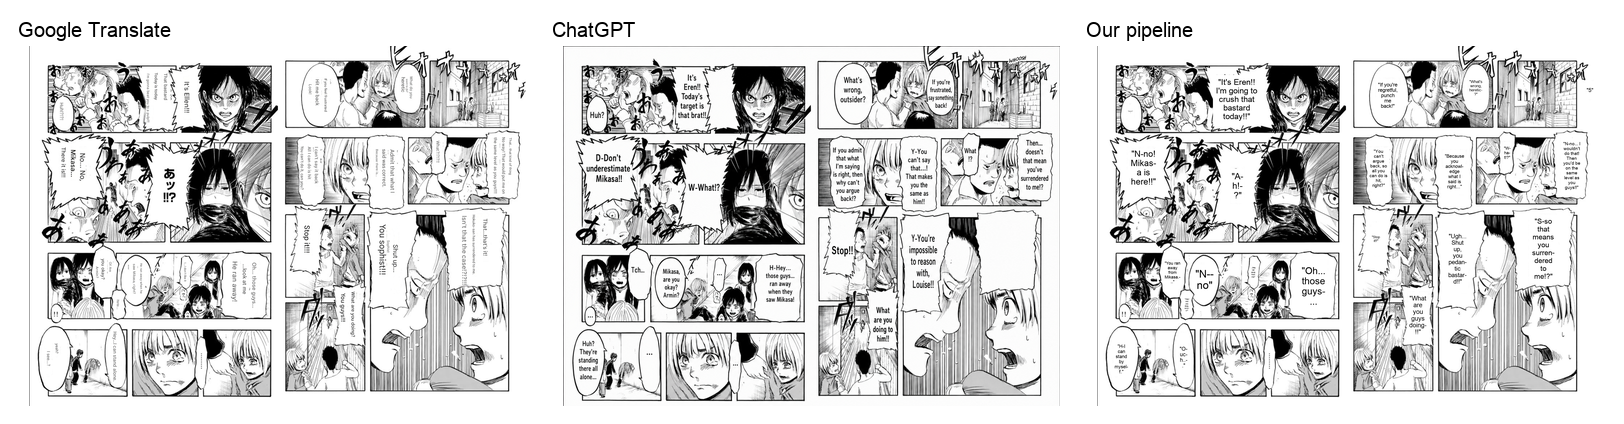
\includegraphics[width=0.98\linewidth]{figures/attack_on_titan_three_way.png}
    \caption{Whole page comparison on \emph{Attack on Titan}: Google Translate, ChatGPT, and our pipeline.}
    \label{fig:aotthreeway}
\end{figure}

\begin{figure}[H]
    \centering
    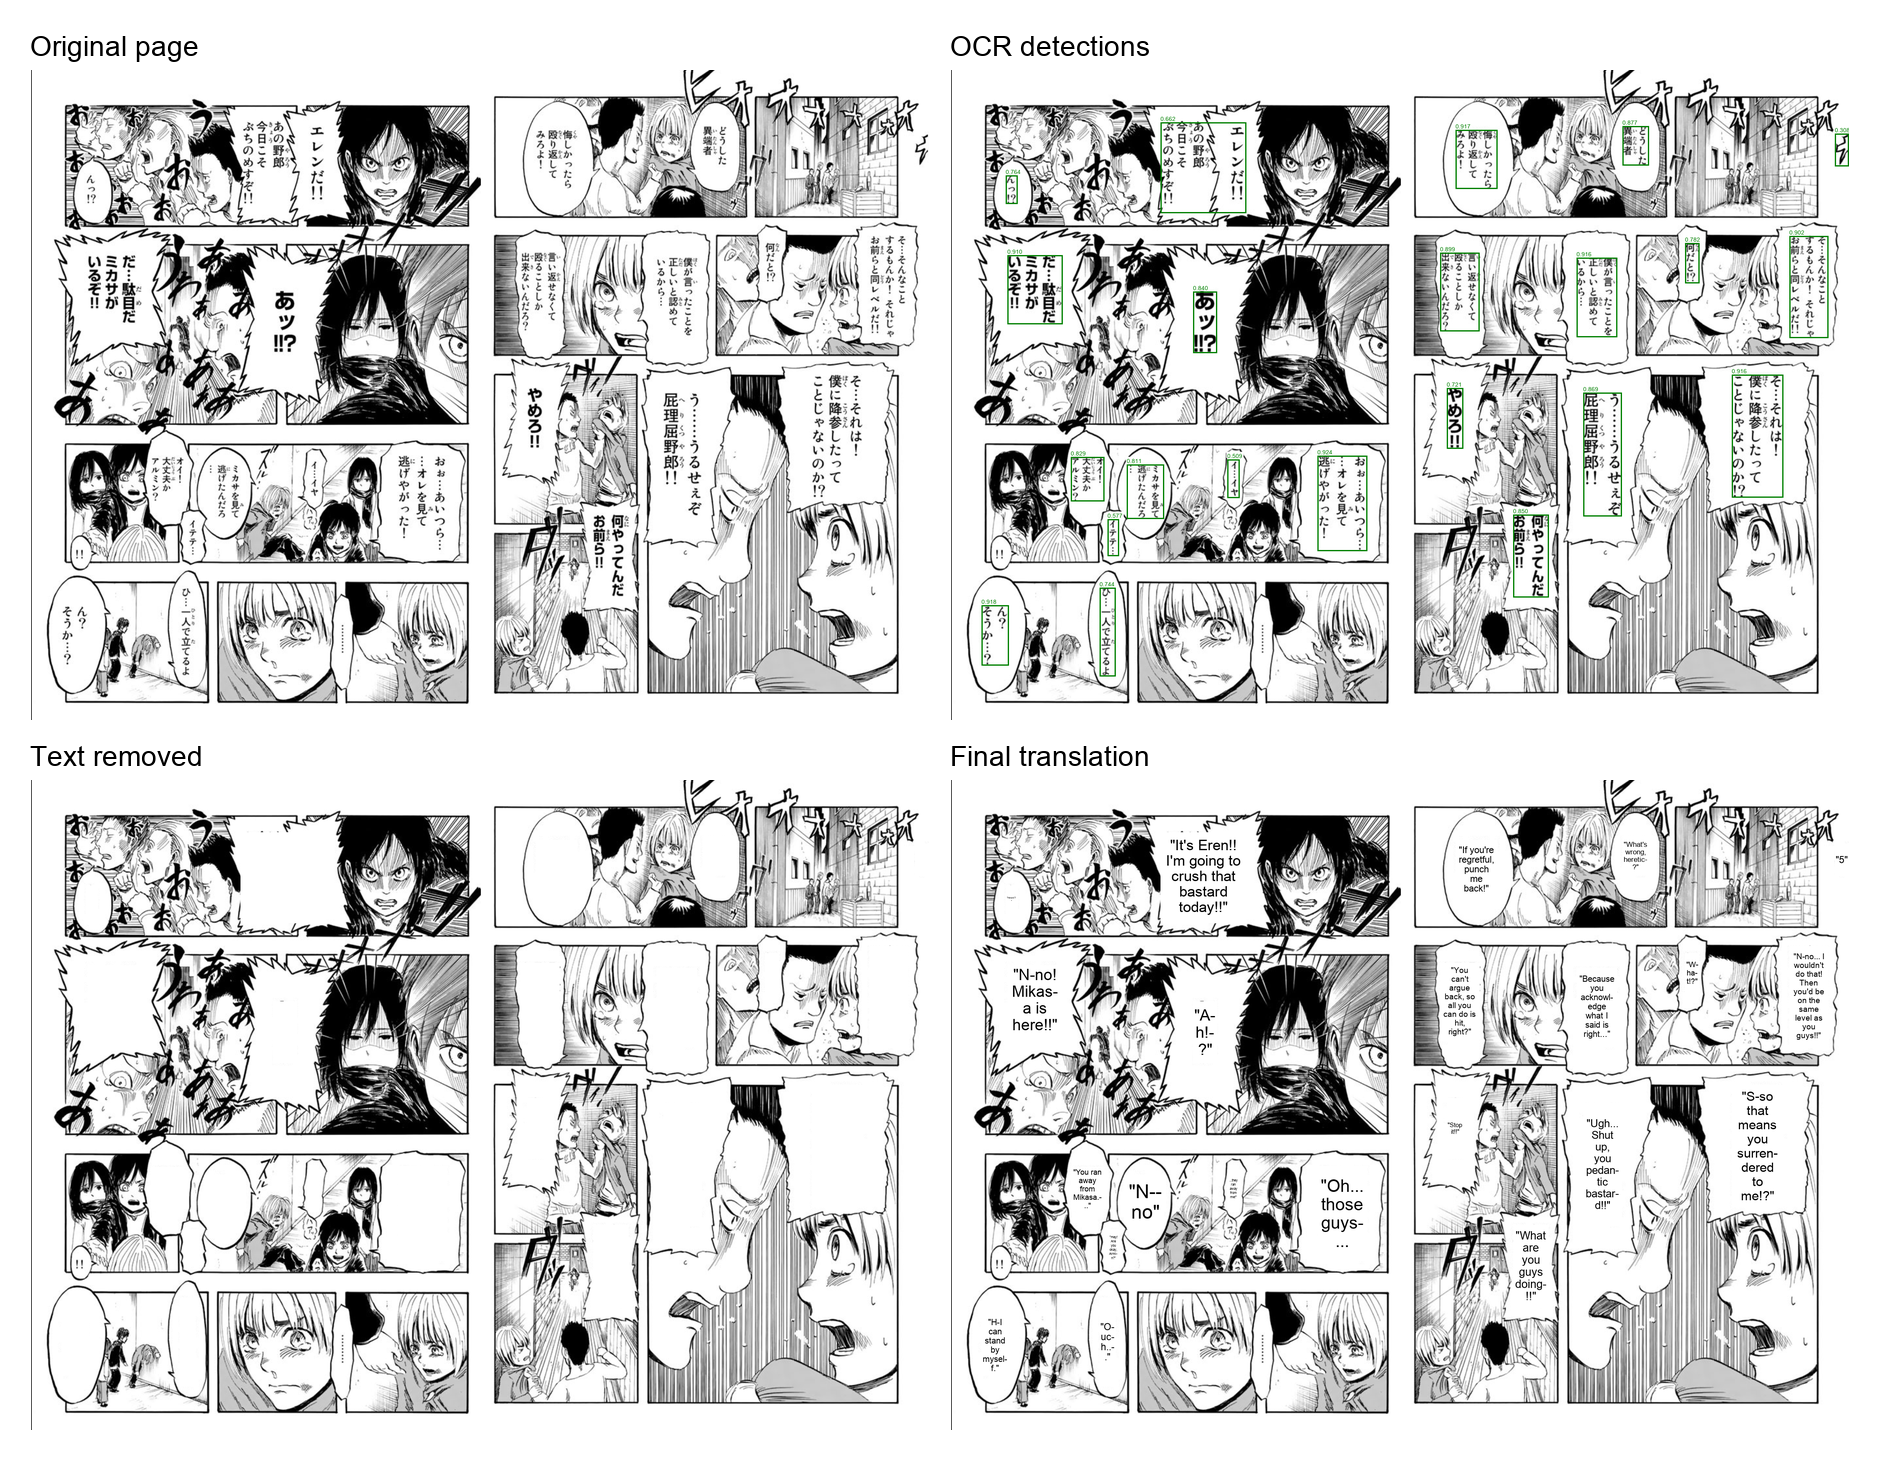
\includegraphics[width=0.98\linewidth]{figures/pipeline_overview.png}
    \caption{Pipeline stages on an \emph{Attack on Titan} page: original image, OCR detections, simple text removal, and final result.}
    \label{fig:pipeline}
\end{figure}

This design was chosen deliberately. Separating OCR from translation makes it possible to measure where errors come from. Running translation on OCR text instead of on the image itself keeps the system more robust: we use a specialized model for detection and extraction, and another for translation, utilizing the strength of each one. Additionally, a dedicated OCR model gives us the bounding boxes which we can \textbf{(a)} use to measure how good detection and extraction is in the results, and \textbf{(b)} use detected bounding boxes in the redraw step, while a pure vision LLM would just give us back translations, without knowing where on the page to place them. The redraw stage is intentionally simple and deterministic: it does not try to reconstruct background art, but it produces a clean and readable result.

\subsection{OCR}
The OCR stage uses PaddleOCR-VL 1.5. It returns page elements with bounding boxes, labels, and confidence values. I only keep text regions and filter very low confidence detections. The threshold is set at 0.2, as otherwise there are a lot of false negatives; there are hardly any false positives. This step is the backbone of the entire system: if a region is missed, it cannot be translated later; if it is transcribed incorrectly, the translator receives corrupted Japanese. The OCR output is also reused for evaluation, debugging, and final rendering, which is why the system stores both raw OCR artifacts and bounding box visualizations.

\subsection{Translation}
Each page is translated from the OCR text only. The translator receives all detected OCR segment from an image and is instructed to return the same number of English segment in the same order, separated by a delimiter. This design makes it easy to map translations back to the correct bubbles. Structured output could have been used instead of a delimiter, but given the simplicity of the task, a simple separator was sufficient. Most of the problems arose due to other problems, described in the results section.

I tried including the original image in the prompt to improve translation quality, but surprisingly, the results did not improve at the expense of the whole pipeline becoming more volatile. The model sometimes disregarded the extracted text in favor of the image, which led to unusable output. As the translation quality did not improve much, the image was remove and only the extracted text was used as input. It is worth noting that this might not be the case had I used a more powerful model such as \texttt{gpt-5.5}.

The LLM is run with deterministic decoding to reduce randomness and improve reproducibility. I also added a benchmark failsafe: if the number of returned translations does not match the number of OCR regions, the benchmark does not crash. Instead, it records a diagnostic status such as \texttt{failed\_empty\_output} or \texttt{count\_mismatch\_missing\_outputs}. This is important for running the full dataset and reporting failure modes.

\subsection{Text removal and redraw}
After OCR, the detected text boxes are filled with white rectangles and the translated English is wrapped and centered inside each region. This is much simpler than true image inpainting or style transfer, but it has two advantages: it is fast, and it makes the output easy to read. The main weakness is that the final page still looks like a cleaned and redrawn page rather than a professionally typeset manga page. Long English lines can also be awkward to fit into narrow vertical bubbles, producing some unpleasant looking word breaks.

\section{Experimental setup}
I evaluated the pipeline on the OpenMantra benchmark, which contains 214 Japanese manga pages with region level bounding boxes and English reference translations. Detection was evaluated with IoU $\geq 0.5$ matching, OCR with character error rate (CER) on matched regions, and translation with BLEU and chrF on matched regions. I also report \emph{end-to-end coverage}, defined as the fraction of all ground truth text regions that make it through the full pipeline with a non empty English output. All experiments were run locally on Apple M3 hardware.

\section{Results and discussion}
Table~\ref{tab:results} summarizes the main benchmark results.

\begin{table}[H]
\centering
\caption{OpenMantra benchmark results.}
\label{tab:results}
\begin{tabular}{lr}
\toprule
Metric & Value \\
\midrule
Pages & 214 \\
Ground truth text regions & 1592 \\
Predicted text regions & 1615 \\
Matched regions & 614 \\
Detection precision & 0.380 \\
Detection recall & 0.386 \\
Detection F1 & 0.383 \\
OCR CER & 0.088 \\
OCR exact match rate & 0.477 \\
Translation BLEU & 19.42 \\
Translation chrF & 38.72 \\
End-to-end coverage & 0.360 \\
Average runtime per page & 6.85 s \\
\bottomrule
\end{tabular}
\end{table}

The most important conclusion is that \textbf{text detection is the main bottleneck}. OCR quality on matched regions is reasonably good: a CER of 8.82\% shows that once the system finds a text region, the Japanese transcription is often usable. Translation quality on those matched regions is also acceptable for a lightweight local system. However, the recall of the detection stage is only 0.386, which means a large amount of dialogue is never passed downstream. End-to-end coverage makes this explicit: it is the share of all ground truth regions that survive detection, OCR, and translation with a non empty English output, which was $573/1592 = 0.360$. It is worth noting that a recall of 0.386 at 0.5 IoU is due to the OCR model not outputting ideal bounding boxes: in many cases, the Japanese text that was outside the bounding box can still be seen, while its whole transcription has been meaningfully translated; in other words, detection is effectively better than the numbers suggest.

The translation stage was mostly stable but not perfectly robust. If pages with no OCR are counted as acceptable skips, then \textbf{13 of 214 pages} had a translation count that did not match the anticipated number of outputs. The breakdown is 7 pages with too few translations, 4 pages with no translation output at all, and 2 pages with too many translations. The 5 \texttt{skipped\_no\_ocr} pages are not counted as translation failures here, because those pages also contain zero ground truth text regions.

In region terms, the translator produced 1556 outputs for 1615 OCR regions, so 62 expected translations were missing and 3 extra translations were produced. The most common failure mode by \emph{page count} was too few outputs, but the biggest loss by \emph{missing regions} came from the 4 empty output pages, which account for 40 of the 62 missing translations. Inspection of the saved outputs suggests that the main underlying reason is alignment brittleness: OCR boxes are region level fragments, not clean sentence units, so the LLM sometimes merges adjacent fragments into one English line, stops early on dense pages, or duplicates a short interjection. So the main issue is not usually that the English itself is bad, but that box level OCR segmentation and line by line generation do not always stay perfectly aligned.

Qualitatively, the system produces readable pages when OCR is clean. On the \emph{Attack on Titan} and \emph{Spy x Family} samples, my output is visually more uniform than the Google Translate image output: the bubbles are explicitly cleaned, the English text is centered, and the result reads more like a re-typeset page. Google Translate often preserves more of the original bubble orientation, but it also tends to insert very small, rotated, or fragmented snippets of English that are harder to read as a finished comic page.

At the same time, Google appears more robust on difficult recognition cases. The \emph{Demon Slayer} sample shows the main weakness of the proposed pipeline: OCR errors propagate directly into translation. In that example, the OCR text contains corrupted characters, and the final English sentence becomes semantically wrong even though the redraw itself still looks clean. Figure~\ref{fig:qualitative} shows the whole page Google Translate vs. our pipeline comparison on \emph{Demon Slayer} and \emph{Spy x Family}. Especially problematic are pronouns and gender related words, as Japanese often omits subjects and (heavily) relies on context.

\begin{figure}[H]
    \centering
    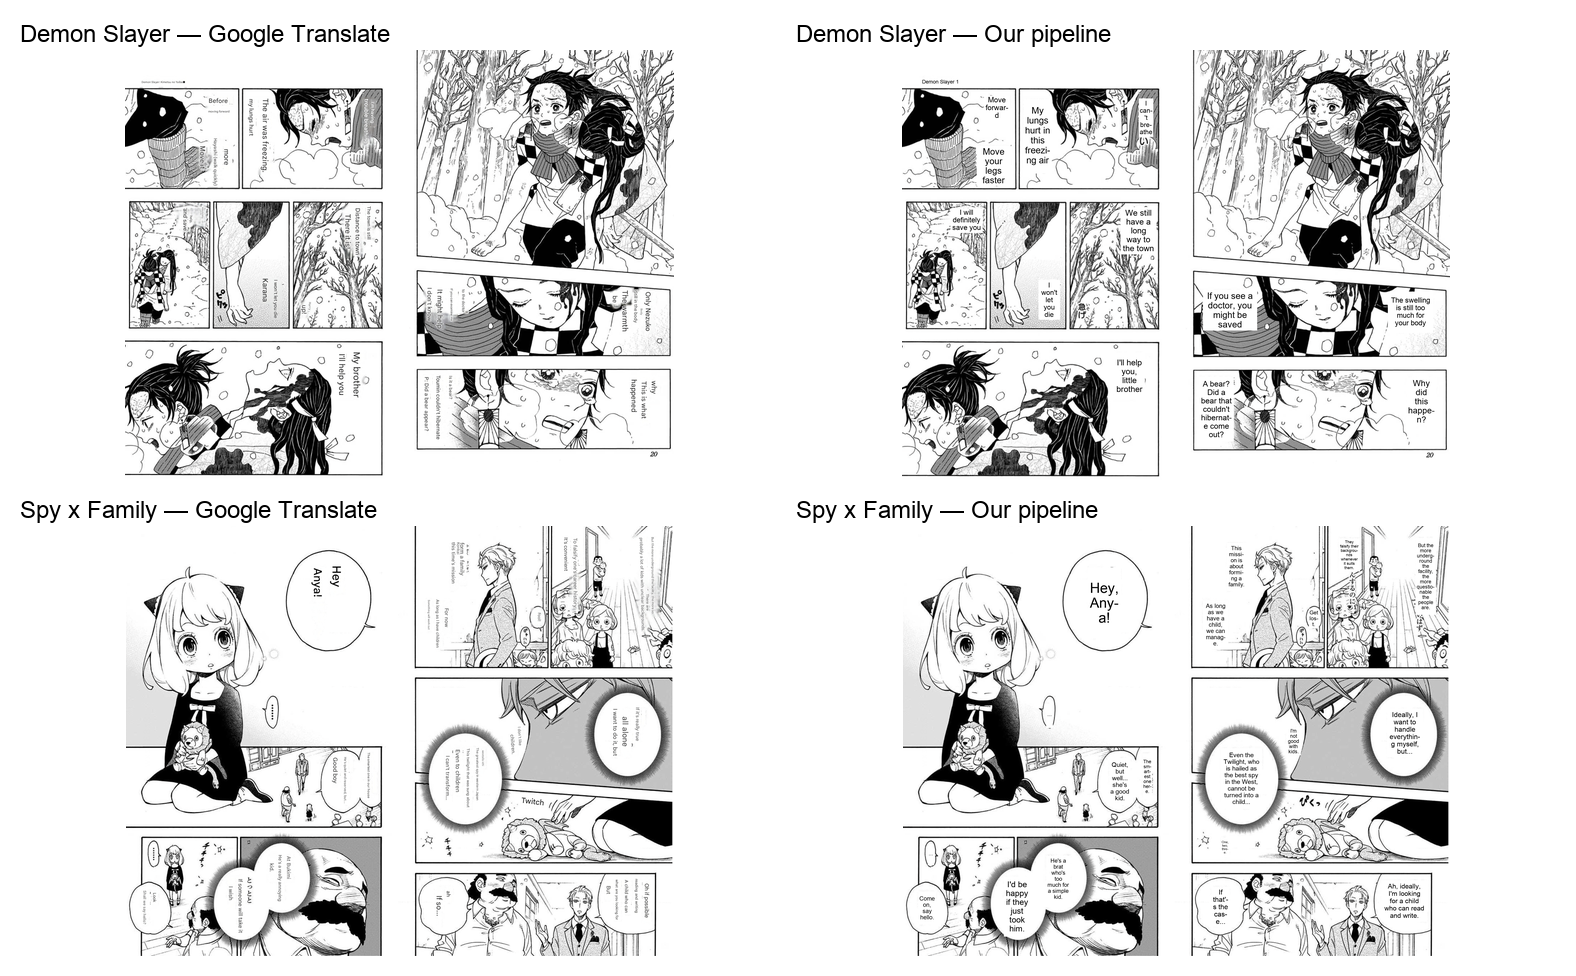
\includegraphics[width=0.94\linewidth]{figures/qualitative_comparison_ds_spy.png}
    \caption{Whole page comparison between Google Translate and our pipeline on \emph{Demon Slayer} and \emph{Spy x Family}. Our output is usually cleaner and more consistent visually, while Google is sometimes more robust on difficult OCR cases.}
    \label{fig:qualitative}
\end{figure}

This makes the benchmark results easy to interpret: the translation model is not the only source of error, and improving OCR would likely help the whole system more than changing the redraw stage. The chosen model, PaddleOCR-VL, is currently SOTA for general purpose OCR, but it was not (presumably) specifically trained on manga text, so it could be further improved with fine-tuning.

A final note on comparison: the OpenMantra paper reports a Google Translate baseline of BLEU 8.72 for Japanese-to-English translation from gold text. That is a useful external reference, but it is not directly comparable to my result because my evaluation is end-to-end on matched OCR regions rather than on ground truth Japanese inputs. For this reason, the image level Google comparison in this report should be treated mainly as a qualitative baseline.

\section{Conclusion}
This project implemented a complete local pipeline for manga translation: OCR, text translation, text removal, and English redraw. The main strengths of the system are modularity, reproducibility, and visually clean redraws on pages where OCR succeeds. The main weakness is limited end-to-end coverage caused by missed or noisy text detection. The benchmark shows that the current system can already produce readable translated pages, but it is not yet robust enough to translate entire manga chapters reliably without omissions.

The clearest next step is therefore not a more complex redraw model, but better text region detection and more robust OCR, ideally combined with stronger handling of vertical text, sound effects, and reading order. After that, the most promising improvement would be a more context aware translation stage that can use panel or page context rather than isolated OCR strings.

Further quality of life improvements could include image inpainting using generative models to reconstruct the background art after text removal (instead of having an ugly looking white cutout), more sophisticated algorithm for determining the best size and position of the translated text, and to support translating into languages other than English.

\section*{References}
\begin{enumerate}[leftmargin=1.5em,itemsep=0pt,topsep=2pt]
    \item C. Morishita et al., ``Towards Fully Automated Manga Translation,'' AAAI, 2021.
    \item PaddleOCR-VL documentation and model release, PaddlePaddle, 2024--2025.
    \item Gemma 4 documentation and model release, HuggingFace (https://huggingface.co/google/gemma-4-E4B-it), 2024--2025.
    \item J. Sachdeva et al., ``The Manga Whisperer,'' CVPR, 2024.
\end{enumerate}

\end{document}
